\newpage
\section{Growing the box}
\genHeader
\hypertarget{sec:growBox}{}

In this SDM, we shall explicitly specify how our learning box is to be built up. We create a specific pattern that will append new partition elements
to the end of \texttt{Box} which will follow our established movement rules (Fig.~\ref{fig:membox_depiction}) for a \texttt{Card}. This means the new partition
will become the \texttt{next} reference of the absolute last partition, and its \texttt{previous} reference must connect to the absolute first partition in the
box (Fig.~\ref{fig:goal_grow}).

\begin{figure}[htbp]
 	\centering
  	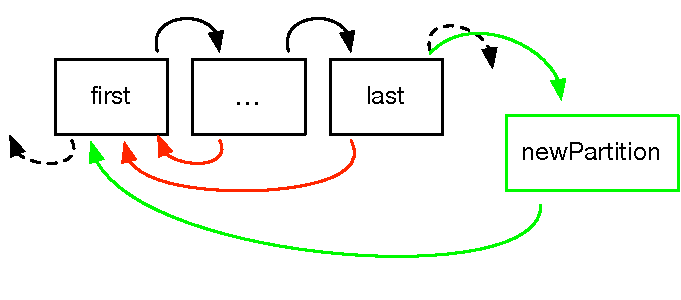
\includegraphics[width=0.7\textwidth]{growBoxNACGoal.pdf}
	\caption{Growing a box by inserting a new partition}
	\label{fig:goal_grow}
\end{figure}
\FloatBarrier

Unfortunately, precise instructions such as these contradict the pattern matcher. We know that, no matter what, a box will always be able to
define first and last partitions. As explained in \hyperlink{sec:emptyPartition}{section 5} however, these will be determined non-deterministically. They will
be chosen at random, and are unlikely to be the actual first and last partitions. How can we guarantee this match to be true?

SDMs provide a declarative means of identifying specific partitions via \emph{Negative Application Conditions}, simply referred to as
\mbox{NAC}s.\footnote{Pronounced $\backslash 'nak \backslash$}\define{NAC}\mbox{NAC}s express structures that are forbidden to exist before or after applying a
transformation rule. In this SDM, the \mbox{NAC} will be a link variable that may not be valid during the pattern match. In the theory of algebraic
graph transformations \cite{EEPT06}, \mbox{NACs} can be complex graphs that are much more general and powerful but in our implementation,\footnote{To be
precise, in CodeGen2 from Fujaba} we only support single negative elements (object or link variables).

As depicted in Fig.~\ref{fig:goal_grow}, to create an appropriate \mbox{NAC} that constrains possible matches, we'll need to check to see if the current matched
pattern has certain `active' link variables. Suppose the targeted last partition has a set \texttt{next} reference. This means it is \emph{not} the absolute
last partition, and so the match becomes invalid. We only want the pattern to insert a new partition when the \texttt{next} link is null. Similarly, if the
targeted first partition has a \texttt{previous} value, the match is invalid. The complete pattern match is therefore made unique through NACs and thus becomes
\emph{deterministic} by construction. In other words, if you \emph{grow} the box with this method, there will always be exactly one first and one last
partition.

Of course, to complete this method we will still need to determine how \emph{many} partitions to add! Since the new size must be calculated depending on the
rest of the partitions currently in the box (partitions usually get bigger) we'll need to call a helper method, \texttt{determineNextSize()}. Instead of declaring this
method with SDMs however, we will expand on injections by writing simple Java code, and generating it into our metamodel.


Previously,\footnote{See Part II, section 5} we learned how to write handwritten code in an implementation file, then generate
a \emph{partial class} to inject code into the metamodel. Now however, we'll generate and edit a partial class to automaticall insert code into the
corresponding Java file, which will then inject into the metamodel.

\begin{itemize}

\item[$\blacktriangleright$] Go to ``BoxImpl.java'' and, without editing any method signatures there, generate its corresponding injection file by either right
clicking the file in the package explorer or within the editor window (Fig.~\ref{}).

\item[$\blacktriangleright$] A second file should now be placed in the \texttt{injection} folder. Open \texttt{BomxImple.inject} and notice the
partial class includes every method declaration but (as expected) no implementation code (Fig.~\ref{fig:injection_partialClassBox}).

\begin{figure}[htbp]
    \centering
    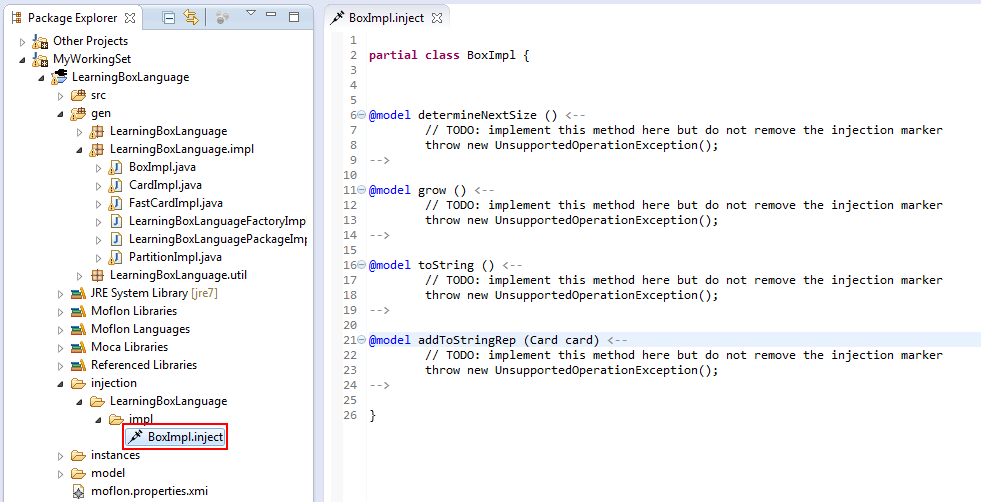
\includegraphics[width=1.0\textwidth]{eclipse_injectionBoxImpl}
    \caption{Generated Injection file for \texttt{BoxImpl.java}}
    \label{fig:injection_partialClassBox}
\end{figure}

\item[$\blacktriangleright$] Complete the \texttt{addToStringRep} and \texttt{determineNextSize} methods as specified in Fig.~\ref{code:complete_inject_file}
below.

\vspace{0.5cm}

\begin{figure}[htbp]
        \centering
        \begin{lstlisting}[language=Java, keywordstyle={\bfseries\color{purple}}, backgroundcolor=\color{white}]
    @model addToStringRep (Card card) <--

            StringBuilder sb = new StringBuilder();

            if (stringRep == null)
            {
                sb.append("BoxContent: [");

            }
            else
            {
                sb.append(stringRep);
                sb.append(", [");
            }

            sb.append(card.getFace());
            sb.append(", ");
            sb.append(card.getBack());
            sb.append("]");

            stringRep = sb.toString();
    -->

    @model determineNextSize () <--

            return getContainedPartition().size() * 10;
    -->

        \end{lstlisting}
        \caption{Implementation of helper methods as an injection}
        \label{code:complete_inject_file}
    \end{figure}
    \FloatBarrier

\vspace{0.5cm}

\item[$\blacktriangleright$] Right-click the injection file, and rebuild your project by selecting ``eMoflon/Clean and
Build''(Fig~\ref{fig:eclipse_buildFromInjecton}).

\item[$\blacktriangleright$] The helper methods should now be implemented in \texttt{BoxImpl.java}, which can be found under
the ``/gen/LearningBoxLanguage.impl'' package (Fig~\ref{fig:eclipse_updatedBoxImpl}).

\item[$\blacktriangleright$] For additional information on injections, check out Part IV: Miscellaneous.\footnote{Download link: \dlPartSix}. Be sure to also
review the work we completed with injections in Part II: Ecore.\footnote{Download Link: \dlPartTwo}

\newpage

\vspace*{2cm}

\begin{figure}[htbp]
    \centering
    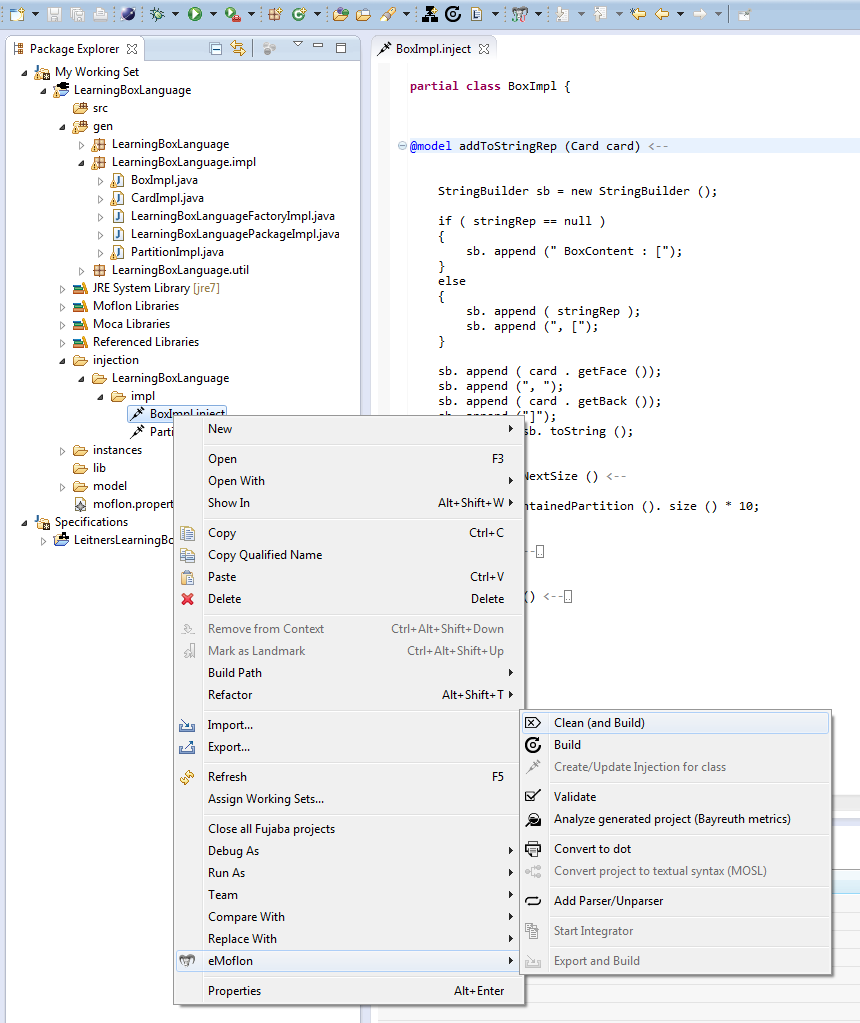
\includegraphics[width=\textwidth]{eclipse_buildFromInject}
    \caption{Build the entire project from the injection file}
    \label{fig:eclipse_buildFromInjecton}
\end{figure}

\newpage

\vspace*{2cm}

\begin{figure}[htbp]
    \centering
    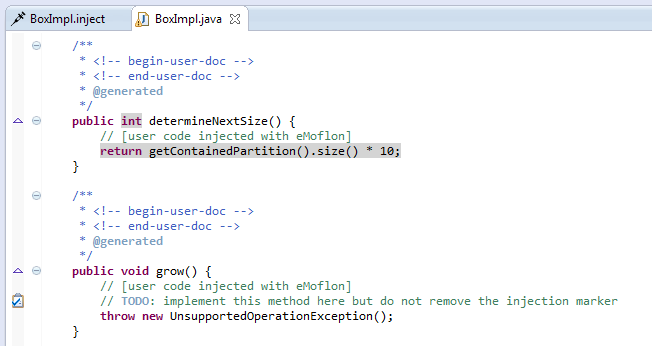
\includegraphics[width=\textwidth]{eclipse_updatedBoxImpl}
    \caption{Updated \texttt{BoxImpl.java} file}
    \label{fig:eclipse_updatedBoxImpl}
\end{figure}

\fancyfoot[R]{ $\triangleright$ \hyperlink{growBox vis}{Next [visual]\hspace{0.2cm} } \\ $\triangleright$ \hyperlink{growBox tex}{Next [textual]} }

\end{itemize}



\newpage
\subsection{Implementing grow}
\visHeader
\hypertarget{growBox vis}{}

\begin{itemize}
 
\item[$\blacktriangleright$] Start by creating the simple story pattern depicted in Fig.~\ref{fig:sdm_grow_1}. This matches the box
(\texttt{this}), with \emph{any} two partitions in the box\footnote{Remember, this is for the \emph{pattern matcher}}.

\begin{figure}[htbp]
\begin{center}
  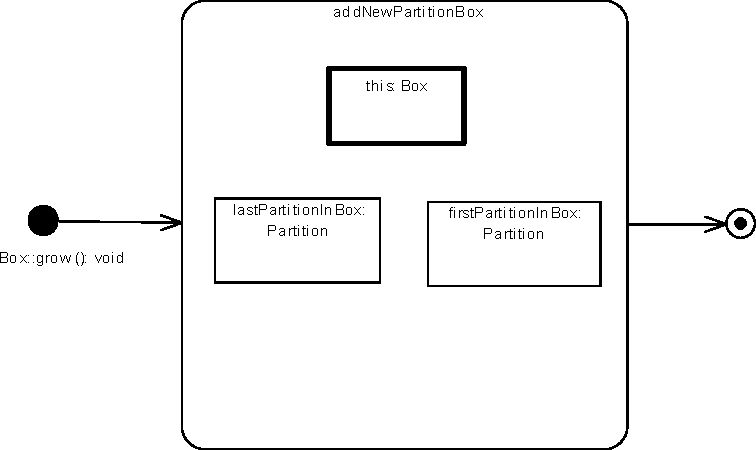
\includegraphics[width=\textwidth]{ea_elementsGrowBox.pdf}
  \caption{Context elements for SDM}  
  \label{fig:sdm_grow_1}
\end{center}
\end{figure}

\item[$\blacktriangleright$] To create the appropriate \mbox{NAC} (to constrain the possible matches for \texttt{lastPartitionInBox}),  create the new object
variable \texttt{nextPartition}, of type \texttt{Partition}, and set \note{Binding Semantics} its \emph{Binding Semantics} to \texttt{negative}
(Fig.~\ref{fig:sdm_grow_2}). The object variable should be visualised as being cancelled or struck out. % why?
 
\begin{figure}[htbp]
\begin{center}
  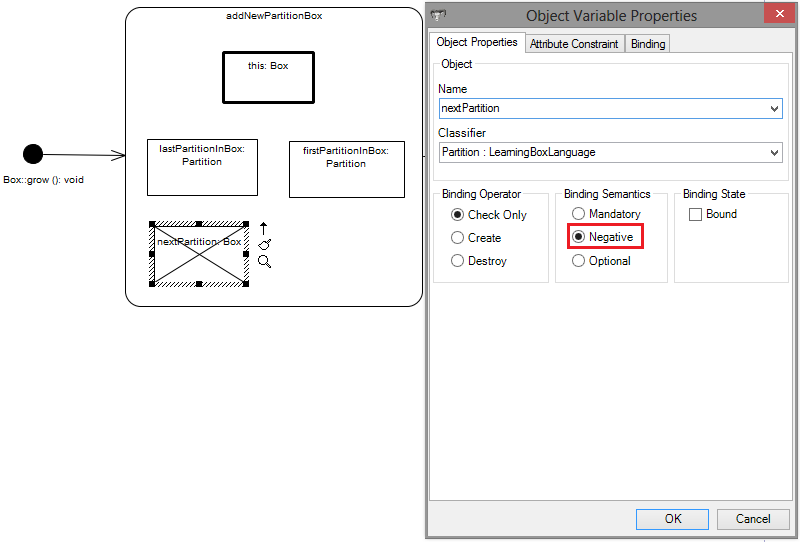
\includegraphics[width=0.9\textwidth]{ea_negElement}
  \caption{Adding a negative element}  
  \label{fig:sdm_grow_2}
\end{center}
\end{figure}
 
\item[$\blacktriangleright$] Now, quick link \texttt{nextPartition} to \texttt{lastPartitionInBox}, but be sure choose the link type carefully! The
\texttt{nextPartition} should play the role of \texttt{next} with respect to \texttt{lastPartitionInBox}.

\item[$\blacktriangleright$] Complete the story pattern so that it closely resembles Fig.~\ref{fig:sdm_grow_3}. 

\begin{figure}[htbp]
\begin{center}
  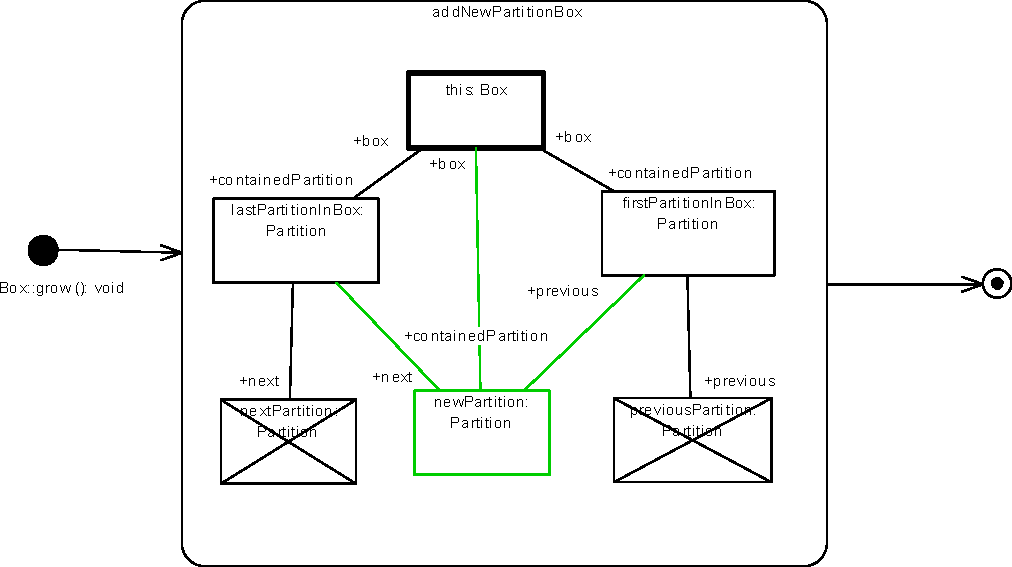
\includegraphics[width=\textwidth]{ea_NACFirstLast.pdf} 
  \caption{Determining the first and last partition with NACs}  
  \label{fig:sdm_grow_3}
\end{center}
\end{figure}
 
\item[$\blacktriangleright$] Notice how the created partition \texttt{newPartition} is `hung' into the box. It becomes the next partition of the current
\emph{last} partition, and has its previous partition set to the first partition in the box (as depicted with the arrows in Fig.~\ref{fig:membox_depiction}).
  
\item[$\blacktriangleright$] To complete this SDM, build the assignment to set the size of the new partition. Go ahead and invoke the corresponding dialogue to
activate the \texttt{:=} operator.

Given that the new size must be calculated using a helper function via a \emph{MethodCallExpression}.\define{MethodCallExpression}A MethodCallExpression is
used to invoke a method defined in any class in the current EA project. Enter the values in Fig.~\ref{fig:sdm_grow_4}, choosing the argument \texttt{this} as
the target, and \texttt{determineNextSize} as the method to be invoked. 

Since \texttt{determineNextSize} doesn't require any parameters, you can ignore the \texttt{Parameters} field this time, but for future reference, parameters
can be specified by choosing the appropriate parameter declaration between guillemets (e.g. \texttt{<Box box>}) found in the drop-down menu and typing in the
value (this is basically a literal expression). Don't forget to press the \texttt{Save} button for every parameter, then \texttt{Add} + \texttt{OK} to confirm
and close the dialogue.
 
 %UPDATE not under 'target' but 'objects'
\begin{figure}[htbp]
\begin{center}
  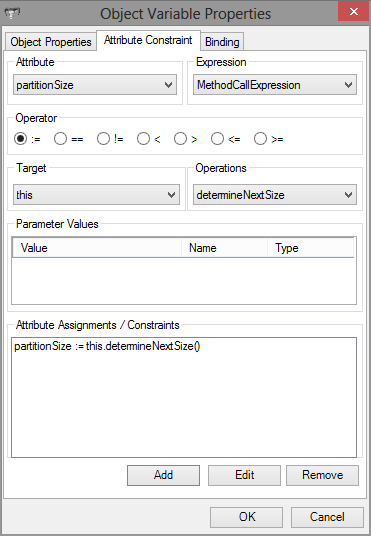
\includegraphics[width=0.5\textwidth]{ea_methodCall.png}
  \caption{Invoking a method via a \texttt{MethodCallExpression} {\bf UPDATE}}  
  \label{fig:sdm_grow_4} 
\end{center}
\end{figure}

\item[$\blacktriangleright$]  If you've done everything right, your SDM should now closely resemble Fig.~\ref{fig:sdm_grow_5}. 

% As usual, try to export, generate code, inspect the
% method implementation and write a JUnit test.  This time around you also have to
% implement the helper method \texttt{determineNextSize} directly in the
% generated code
% (\texttt{gen/\-LearningBoxLanguage/\-facade/\-impl/\-LearningBoxUtilImpl}).
% Don't forget to add \texttt{@generated NOT} to the Java doc comment of the
% method so the code generator preserves your code in future runs.
% When testing (which you will \emph{of course} do right?), note that you can only grow a ``minimal'' box that has at least a first and last partition, i.e., a box with 
%no partitions at all cannot be grown using our specified SDM. 

\begin{figure}[htbp]
\begin{center}
  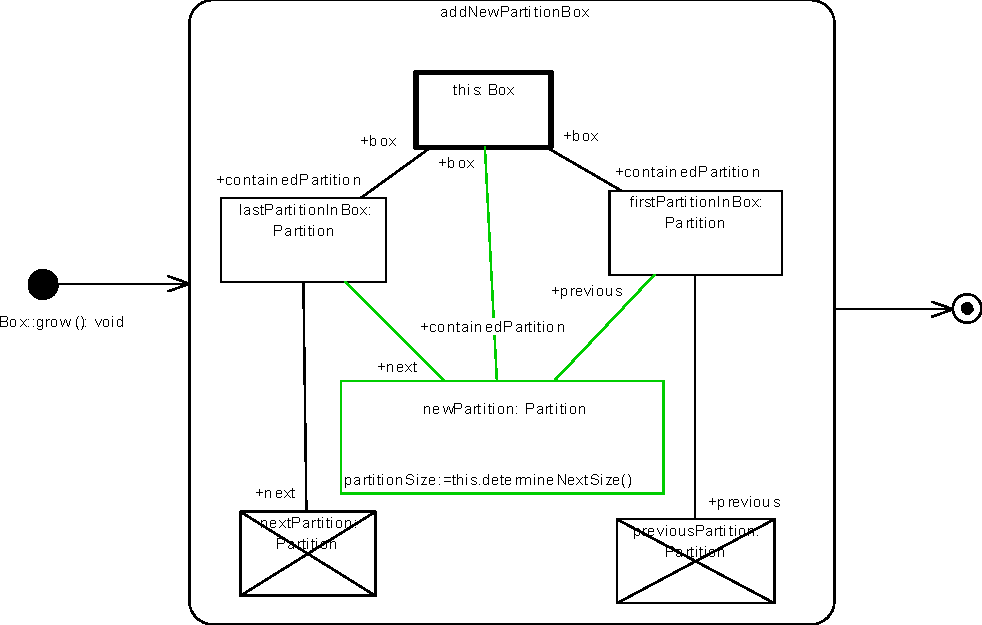
\includegraphics[width=0.9\textwidth]{ea_completeActivityGrowBox.pdf}
  \caption{Complete SDM for \texttt{Box::grow}}  
  \label{fig:sdm_grow_5}
\end{center}
\end{figure}

\item[$\blacktriangleright$]  That's it - your \texttt{grow} SDM is complete! This was probably the most challenging SDM to build, so give yourself a solid 
pat on the back. If you found it easy then \ldots gee whiz, I don't think i'm doing my job correctly. To see how this is done in the texual syntax, review
Fig.~\ref{fig:patternComplete}.\footnote{We do recommend reading the instructions for this one, however, since NACs can be tricky.}

\end{itemize}


\clearpage
\hypertarget{growBox tex}{}
\subsection{Implementing grow}
\texHeader

\vspace*{0.5cm}

\begin{itemize}

\item[$\blacktriangleright$] In \texttt{box.grow()}, create a simple control flow with one story pattern (Fig.~\ref{fig:growDecl}). 

\begin{figure}[htbp]
\begin{center}
  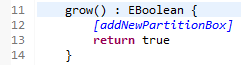
\includegraphics[width=0.4\textwidth]{eclipse_growDecl}
  \caption{Basic control flow to grow \texttt{box}}
  \label{fig:growDecl}
\end{center}
\end{figure}

\item[$\blacktriangleright$] Create and open the new pattern. You'll want it to match the invoking box with \emph{any} two partitions, so create a bound
\texttt{this} box, and the free variables \texttt{firstPartitionInBox} and \texttt{lastPartitionInBox}. You'll also need an object variable (set to create) to
represent the new partition. The skeleton of your pattern should now resemble (Fig.~\ref{fig:growPattSkel}).

\vspace{0.5cm}

\begin{figure}[htbp]
\begin{center}
  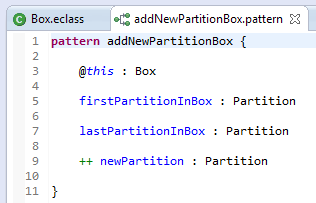
\includegraphics[width=0.5\textwidth]{eclipse_growPatternSkeleton}
  \caption{The \texttt{addNewPartitionBox} skeleton}
  \label{fig:growPattSkel}
\end{center}
\end{figure}

\item[$\blacktriangleright$] Next, we need to create an appropriate \emph{NAC} which will constrain the possible choices for \texttt{lastPartitionInBox}.
Create a negative \texttt{next\-Part\-it\-ion} object variable by using the negation `!' operator.

\vspace{0.5cm}

\item[$\blacktriangleright$] Now add \texttt{`->next : nextPartition'} to \texttt{lastPartition}'s scope. This attempts to establish a \texttt{next} link from
the last partition. Next, add \texttt{`++ ->next : newPartition'} (Fig.~\ref{fig:firstNAC}). This constraint will only be fulfilled if the NAC fails, and it
establishes the \texttt{newPartition} as the final partition.

\begin{figure}[htbp]
\begin{center}
  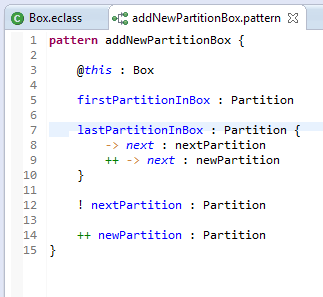
\includegraphics[width=0.5\textwidth]{eclipse_growLastNAC}
  \caption{Creating the first NAC \update}
  \label{fig:firstNAC}
\end{center}
\end{figure}

\vspace{0.5cm}

\item[$\blacktriangleright$] In a similar fashion, create a second NAC, \texttt{previousPartition}, for \texttt{firstPartitionInBox}. No new references have to
be created here, so all you need to establish is the link connecting \texttt{firstPartitionInBox} to the negative element, \texttt{previousPartition}
(Fig.~\ref{fig:growPatt}).

\begin{figure}[htp]
\begin{center}
  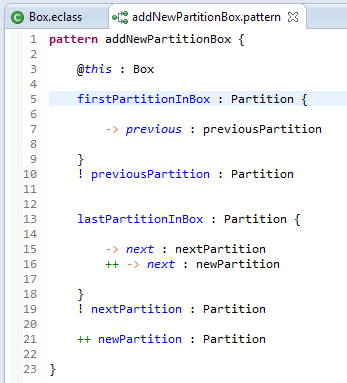
\includegraphics[width=0.55\textwidth]{eclipse_growFirstNAC}
  \caption{Pattern with both NACs}
  \label{fig:growPatt}
\end{center}
\end{figure}

\item[$\blacktriangleright$] Now edit \texttt{@this} with appropriate link variables to the first and last partitions. Try using auto-completion here for the
reference names!

\newpage

\item[$\blacktriangleright$] The next step is to establish the \texttt{box} and \texttt{previous} references in our newly created object variable,
\texttt{newPartition}. While you could of course write \texttt{`++ ->box : this'}, any link variables established here are automatically set to `green,' and do
not need to be explicitly set with an \texttt{++} operator. This is because you cannot connect a `black' link to a `green' node.\footnote{Remember that a rule
actually consists of two graphs: r = (L,R). A green node only belongs to R and not to L, while a black link is in L and in R. If the target of the link is only
in R, however, L would have a link with an undefined target. This is not allowed (L is not a graph).} In other words, a `green' object variable has a global
effect on all link variables declared in its scope.

\item[$\blacktriangleright$] Your pattern should now resemble Fig~\ref{fig:growAllLinks}. 

\begin{figure}[htp]
\begin{center}
  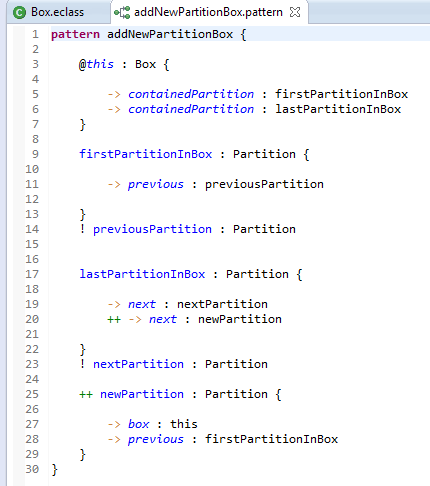
\includegraphics[width=0.65\textwidth]{eclipse_growLinks}
  \caption{Pattern  with deterministic choice of first and last partitions}
  \label{fig:growAllLinks}
\end{center}
\end{figure}

\item[$\blacktriangleright$] We're not \emph{quite} done yet - our newest partition doesn't yet have a size. This means that not only do we need to make
another attribute constraint to set its value, but \texttt{newPartition} needs to directly invoke a method in order to get the correct value. You can do this
via a \emph{MethodCallExpression}. The structure of this expression is similar to Java where:
\syntax{MethodCallExpression := (object\_variable\_expression | \\ parameter\_expression)`.'ID`('argument\_list `)'}

\item[$\blacktriangleright$] We've encountered both of these expression types already -- \texttt{`@'} in \texttt{removeCard} and \texttt{`\$'} in
\texttt{check}. The latter doesn't apply to this pattern, so write: \syntax{@this.determineNextSize()}.

\item[$\blacktriangleright$] Your workspace should now resemble Fig.~\ref{fig:patternComplete}.

\vspace{0.5cm}

\begin{figure}[htp]
\begin{center}
  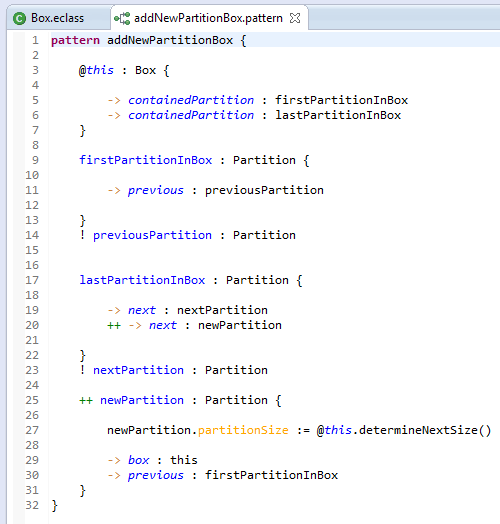
\includegraphics[width=0.9\textwidth]{eclipse_growFinished}
  \caption{Complete pattern for adding a new \texttt{partition} to \texttt{Box}}
  \label{fig:patternComplete}
\end{center}
\end{figure}

\vspace{0.5cm}

\item[$\blacktriangleright$] \emph{Now} we're done! While NACs may be difficult to understand at first, as you can see, they're not hard to implement, and
can be used in a wide variety of applications. To see how this method is implemented in the visual syntax, check out Fig.~\ref{fig:growComplete} in the
previous section.

\end{itemize}
